\section{Where Does Gravity Come From?}
\label{sec:gravity_distance}

\subsection{The Distance of Vol.1 and Its Limitation}

In Vol.~1, distance was defined purely from the causal log structure:
\begin{equation}
  d_{ij} = -\log \tilde{S}_{ij},
  \qquad
  \tilde{S}_{ij} = \max_{\gamma: i\to j} \prod_{(ab)\in\gamma} S_{ab}.
\end{equation}
This definition selects the path of maximal propagation strength.
Distance is therefore determined by the most permeable structural path.
\begin{equation}
  \boxed{\text{Distance is determined solely by the structure of } C_{ij}.}
\end{equation}
This construction yields a consistent geometry derived entirely from
relational structure. However, an important limitation appears.
\begin{equation}
  \boxed{\text{Gravity does not explicitly emerge from this definition.}}
\end{equation}
The reason is that the distance above assumes structural homogeneity.
All regions are treated equally except for variations encoded in propagation strength.
No mechanism exists that biases path selection according to accumulated structure.
Gravity, however, appears precisely as such a bias.

\subsection{What Is Gravity?}

In conventional physics, gravity is introduced either as a force acting between
masses, or as curvature of spacetime. VED adopts a different starting point.
\begin{equation}
  \boxed{
    \text{Gravity is the phenomenon by which closure density distorts
    the distance structure.}
  }
\end{equation}
This represents a shift in perspective.
The conventional approach introduces a new interaction.
VED modifies the definition of distance itself.
\begin{equation}
  \boxed{\text{Gravity is not added. It is a reinterpretation of existing structure.}}
\end{equation}
Thus gravity is not an independent entity, but an emergent bias in the same
structural geometry already defined in Vol.~1.

\subsection{Extension of Distance}

To incorporate this bias, assign a cost to each edge $(a,b)$:
\begin{equation}
  \label{eq:path_cost}
  w_{ab} = -\log S_{ab} + \epsilon\, L_{ab}.
\end{equation}
The first term represents geometric permeability, identical to Vol.~1.
The second term introduces a congestion cost due to closure density.
Distance is then defined by minimizing total path cost:
\begin{equation}
  \boxed{d_{ij} = \min_{\gamma: i\to j} \sum_{(ab)\in\gamma} w_{ab}.}
\end{equation}
This expression unifies geometry and gravitational effect within a single
path selection principle.
The overall structure is summarized in Figure~\ref{fig:gravity_chain}.

\begin{figure}[h]
  \centering
  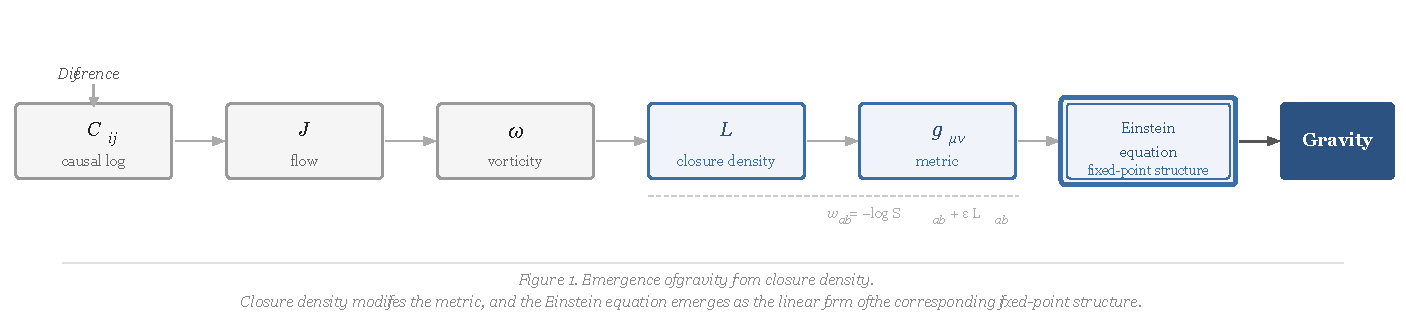
\includegraphics[width=\textwidth]{figures/VED_Vol3_Figure1.pdf}
  \caption{
    Emergence of gravity from closure density.
    Causal logs generate flow and vorticity, which produce closure density.
    Closure density modifies the metric,
    and the Einstein equation emerges as the linear form
    of the corresponding fixed-point structure.
    Gravity therefore emerges as a modification of distance
    rather than a fundamental force.
  }
  \label{fig:gravity_chain}
\end{figure}

\subsection{What the Unified Path Implies}

It is essential that both terms in equation~\eqref{eq:path_cost}
are evaluated along the same path.
If propagation strength and closure density were evaluated on different paths,
the geometry would split into separate structures.
\begin{equation}
  \boxed{\text{Gravity alters path selection itself.}}
\end{equation}
This mirrors the conceptual shift introduced by general relativity.
Einstein replaced force with curvature.
VED replaces curvature with path cost.
The two descriptions differ in interpretation but agree structurally.

\subsection{Summary}

By incorporating closure density into the distance definition,
gravity emerges naturally from the same structural framework.
\begin{equation}
  \boxed{\text{Gravity is not a new force.}}
\end{equation}
\begin{equation}
  \boxed{\text{It appears as a modification of the definition of distance.}}
\end{equation}
